% \begin{chapter}*{}

% \aosafigure{../images/backmatter/making.pdf}{}{fig.making.making}
\thispagestyle{empty}

\sffamily

\Large You May Also Enjoy\ldots

\normalsize

\begin{figure}[h!]
\centering
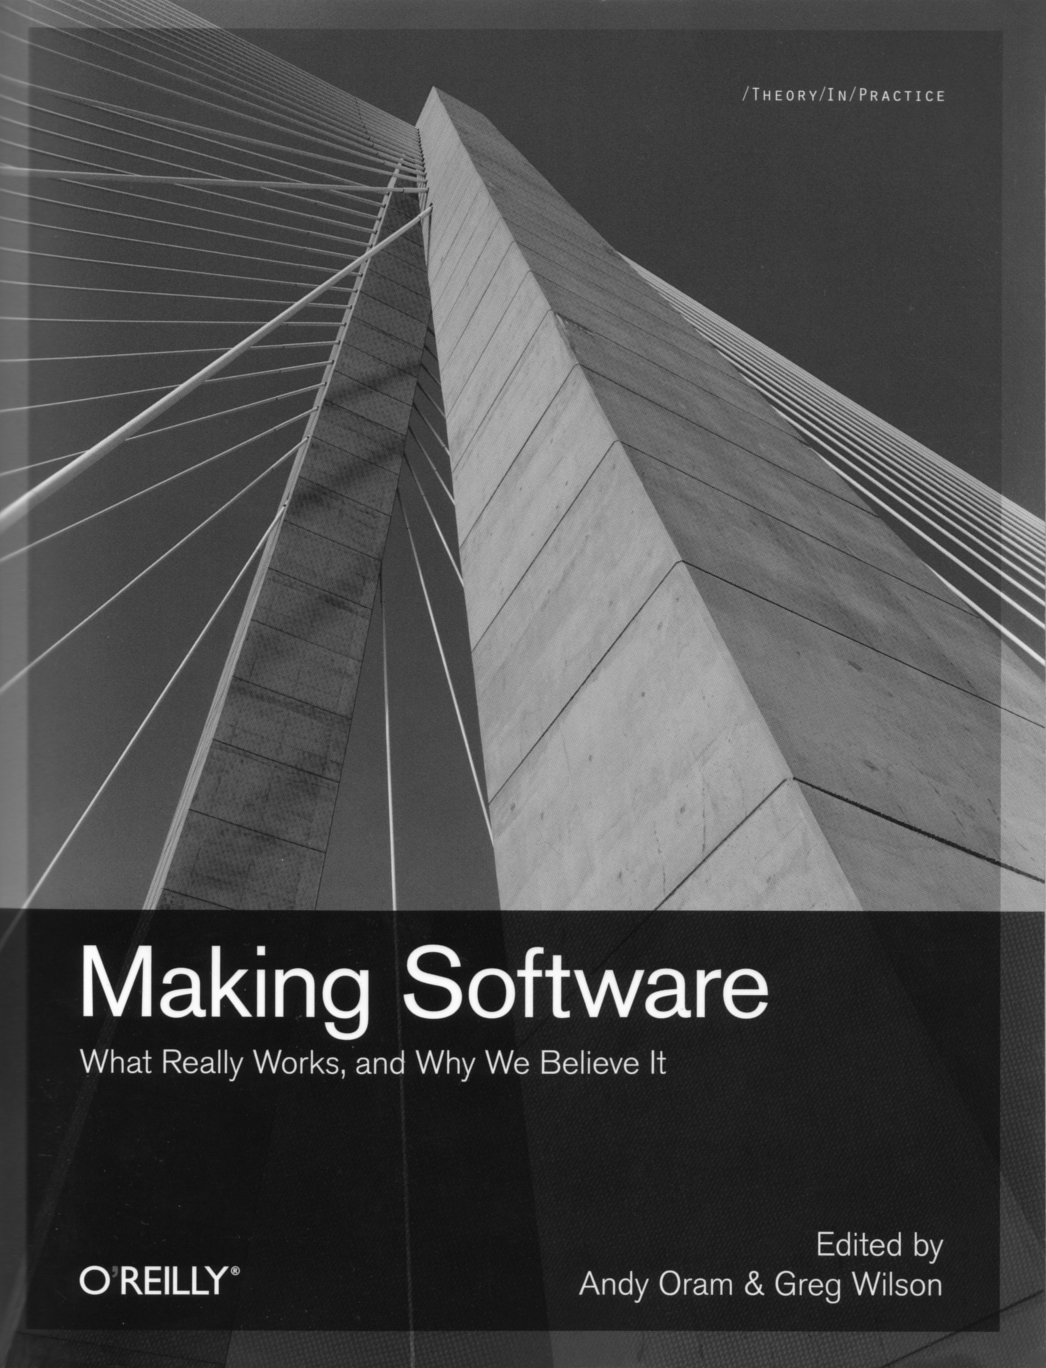
\includegraphics[width=250pt]{../images/backmatter/making.pdf}
\end{figure}

Many claims are made about how certain tools, technologies, and
practices improve software development. But which are true, and which
are merely wishful thinking? In \emph{Making Software}, leading
researchers and practitioners present chapter-length summaries of key
empirical findings in software engineering, and answer questions like:

\vspace{-0.1cm}

\begin{aosaitemize}

\item Are some programmers really ten times more productive than others?

\item Does writing tests first help you develop better code faster?

\item Can code metrics predict the number of bugs in a piece of software?

\item Does using design patterns actually make software better?

\item What effect does personality have on pair programming?

\item What matters more: how far apart people are geographically, or how far apart they are in the org chart?

\end{aosaitemize}

\vspace{-0.2cm}

\setlength{\parskip}{0.15cm}

\noindent As with \emph{The Architecture of Open Source Applications}, royalties
from \emph{Making Software} will be donated to Amnesty International.

\noindent \emph{Making Software: What Really Works, and Why We Believe It} \\
edited by Andy Oram and Greg Wilson \\
O'Reilly Media, 2010, 978-0596808327 \\
\url{http://oreilly.com/catalog/9780596808303}

\normalfont

\pagebreak
\thispagestyle{empty}

